\chapter{Lecture 17: Level Curves \& The Riemann Mapping Theorem}

\section{Level Curves}

\begin{claim}
    [Orthogonal Level Curves]
    Suppose $f = u + iv$ is an analytic function and some $f'(z_0) \neq 0$. Then the level curves of $u$ and $v$ centered around $z_0$ intersect orthogonally at $z_0 = x_0 + iy_0$.
    \begin{align*}
        \gamma_1 & = \{z : u(z) = u(z_0)\} \text{ the set of points in } \mathbb{C} \text{ where real part of } f \text{ is constant}      \\
        \gamma_2 & = \{z : v(z) = v(z_0)\} \text{ the set of points in } \mathbb{C} \text{ where imaginary part of } f \text{ is constant}
    \end{align*}
    This is because at $z_0$ is the only point shared between $\gamma_1$ and $\gamma_2$.
    \begin{figure}[H]
        \centering
        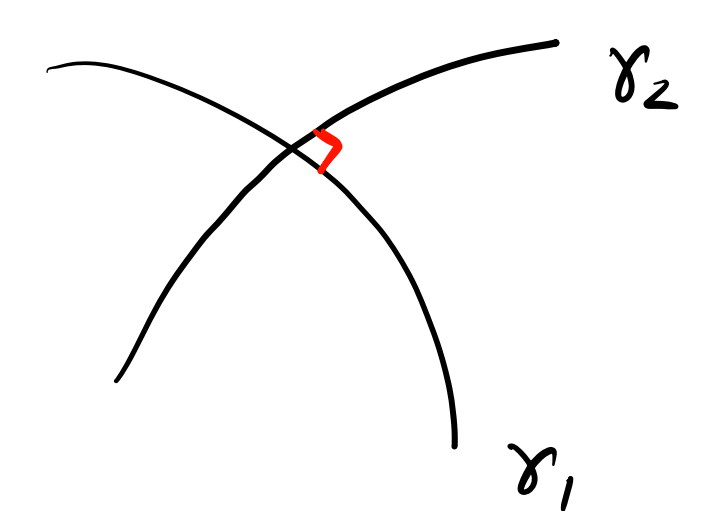
\includegraphics[width=0.5\textwidth]{LECTURE_17/graph.png}
        \caption{Level Curves}
    \end{figure}
\end{claim}

\begin{proof}
    $f$ is a conformal map and $\gamma_1, \gamma_2$ are curves in $\mathbb{C}$ such that $\gamma_1(0) = \gamma_2(0) = z_0$. So the angle between $\gamma_1, \gamma_2$ at $z_0$ is the same as the angle between $f(\gamma_1), f(\gamma_2)$ at $f(z_0)$.
    \begin{itemize}
        \item $f(\gamma_1) = \{w \in \mathbb{C} :\Re (w) = u(z_0)\}$
        \item[$\rightarrow$] $w = f(z)$ for each $z \in \gamma_1$
        \item[] We know for each $z \in \gamma_1$ that $u(z) = u(z_0)$
        \item[] Because $f^{-1}(w) = z$, we have $u(f^{-1}(w)) = u(z) = u(z_0) = \Re (w)$
        \item $f(\gamma_2) = \{w \in \mathbb{C} :\Im (w) = v(z_0)\}$
    \end{itemize}
    \begin{figure}[H]
        \centering
        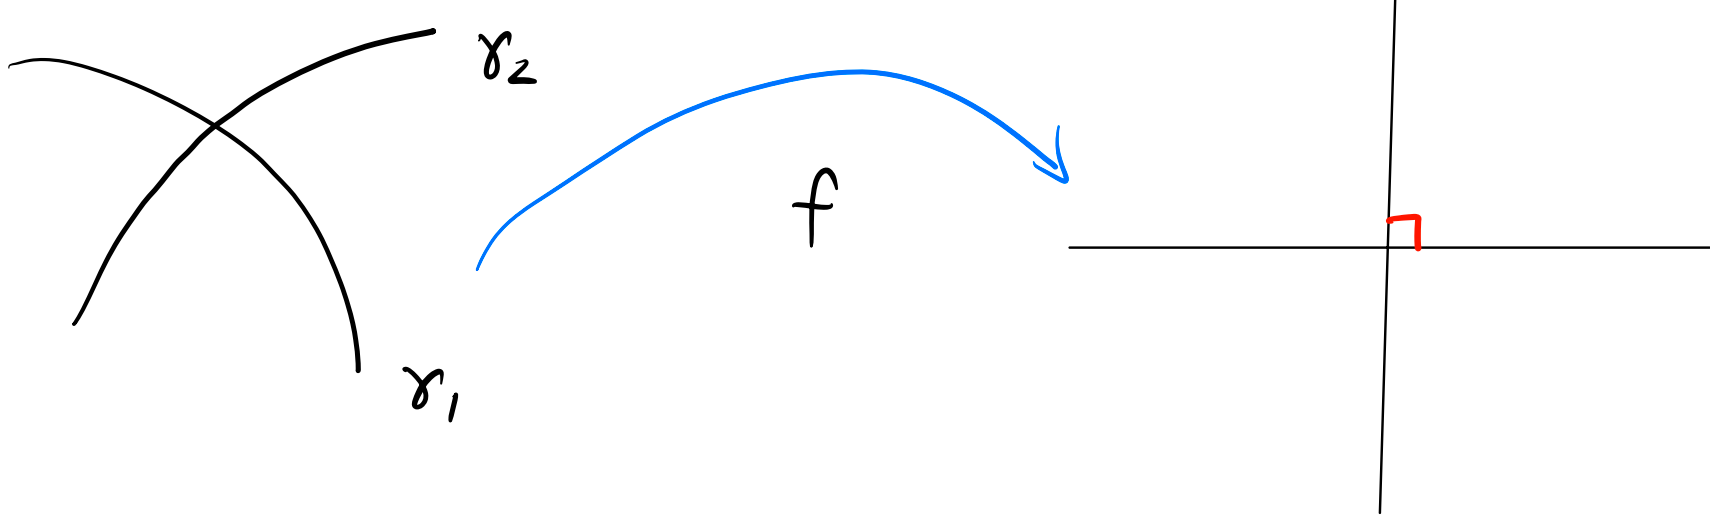
\includegraphics[width=0.5\textwidth]{LECTURE_17/conformal.png}
        \caption{Level Curves under $f$}
    \end{figure}
    Due to the fact that $nabla u \cdot \nabla v = 0$ at every point, this means $f(\gamma_1) = u(z_0)$ and $f(\gamma_2) = v(z_0)$ intersect orthogonally at $f(z_0)$, and thus $\gamma_1, \gamma_2$ intersect orthogonally at $z_0$.
\end{proof}

\begin{example}
    \begin{itemize}
        \item[(i)] $f(z) = e^z = \underbrace{e^x(\cos y)}_u + i\underbrace{e^x(\sin y)}_{v}$
    \end{itemize}
    \begin{figure}[H]
        \centering
        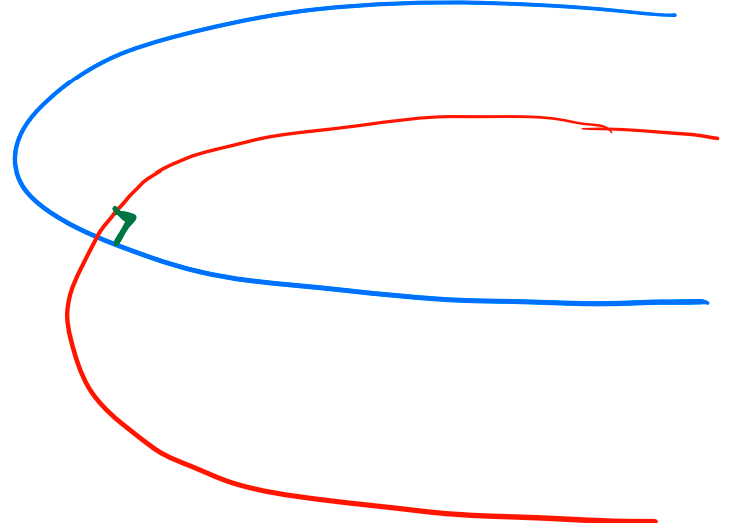
\includegraphics[width=0.5\textwidth]{LECTURE_17/graph1.png}
        \caption{Level Curves of $e^z$}
    \end{figure}
    Let's consider the level curves of $u$ and $v$.
    \begin{align*}
        \gamma_1    & = \{z \in \mathbb{C} : u(z) = u(z_0)\}                   \\
        e^x(\cos y) & = C_1 \quad \text{for some constant } C_1 \in \mathbb{R} \\
    \end{align*}
    If $C_1 = 0$ then:
    \begin{align*}
        e^x(\cos y) = 0 \implies \cos y = 0 \implies y = \frac{\pi}{2} + n\pi
    \end{align*}
    If $C_1 \neq 0$ then:
    \begin{align*}
        e^x(\cos y) = C_1 \implies e^x & = \frac{C_1}{\cos y} \quad \text{for } y \neq \frac{\pi}{2} + n\pi \\
        x                              & = \log \left(\frac{C_1}{\cos y}\right)
    \end{align*}
    So $\gamma_1$ is a set of $z = (x, y)$ such that $x = \log \left(\frac{C_1}{\cos y}\right)$ for $y \neq \frac{\pi}{2} + n\pi$.\\
    Similarly, $\gamma_2$ is a set of $z = (x, y)$ such that $x = \log \left(\frac{C_2}{\sin y}\right)$ for $y \neq n\pi$.\\
    Because $f'(z_0) = e^{z_0} \neq 0$, we can show that the level curves of $u$ and $v$ intersect orthogonally at any point $z_0$.
    \begin{align*}
        \nabla u & = \begin{pmatrix}
                         \frac{\partial u}{\partial x} \\ \frac{\partial u}{\partial y}
                     \end{pmatrix} = \begin{pmatrix}
                                         e^x\cos y \\ -e^x\sin y
                                     \end{pmatrix} \\
        \nabla v & = \begin{pmatrix}
                         \frac{\partial v}{\partial x} \\ \frac{\partial v}{\partial y}
                     \end{pmatrix} = \begin{pmatrix}
                                         e^x\sin y \\ e^x\cos y
                                     \end{pmatrix}
    \end{align*}
    Then we can use the dot product, which is $0$ iff the vectors are orthogonal.
    \begin{align*}
        \nabla u \cdot \nabla v = e^{x}\cos(y)e^{x}\sin(y) - e^{x}\cos(y)e^{x}\sin(y) = 0
    \end{align*}
\end{example}

\begin{example}
    \begin{itemize}
        \item[(ii)] $\text{Log} z = \underbrace{\log |z|}_u + i\underbrace{\text{Arg}(z)}_v$
    \end{itemize}
    \begin{figure}[H]
        \centering
        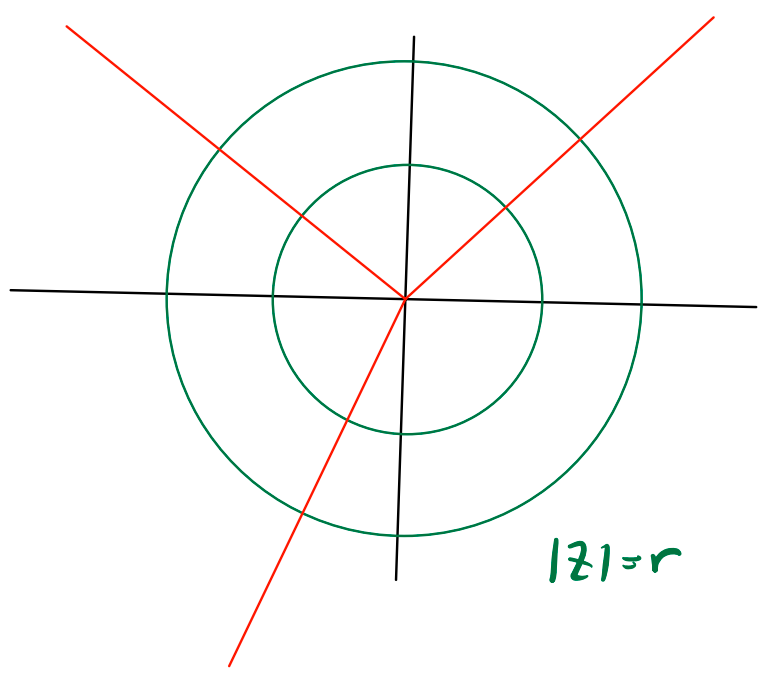
\includegraphics[width=0.5\textwidth]{LECTURE_17/graph2.png}
        \caption{Level Curves of $\text{Log} z$}
    \end{figure}
\end{example}

\section{The Riemann Mapping Theorem}

\begin{theorem}
    [Riemann Mapping Theorem]
    Suppose $D \subset \mathbb{C}$ is a simply connected domain such that $D \neq \mathbb{C}$. Let $p \in D$ be a point in $D$. Then there is a one-to-one analytic function $\phi$ such that:
    \begin{align*}
        \phi : D \to \{w \in \mathbb{C} : |w| < 1\}
    \end{align*}
    and $\phi(p) = 0$. $\phi$ is uniquely determined if we require $\phi'(p) > \mathbb{R}_{> 0}$.\\
    Basically, we can map any simply connected domain to the unit disk.
\end{theorem}

\begin{corollary}
    If $D_1, D_2$ are simply connected domains $D_1 \neq \mathbb{C} \neq D_2$, then $\exists \phi$ that's one-to-one and analytic such that:
    \begin{align*}
        \phi(D_1) = D_2
    \end{align*}
\end{corollary}

\begin{proof}
    $D_1 \xrightarrow{\phi_1} \{w \in \mathbb{C} : |w| < 1\}$ and $D_2 \xrightarrow{\phi_2} \{w \in \mathbb{C} : |w| < 1\}$.\\
    $\phi_2^{-1} \circ \phi_1$ is the desired map.
\end{proof}

\begin{figure}[H]
    \centering
    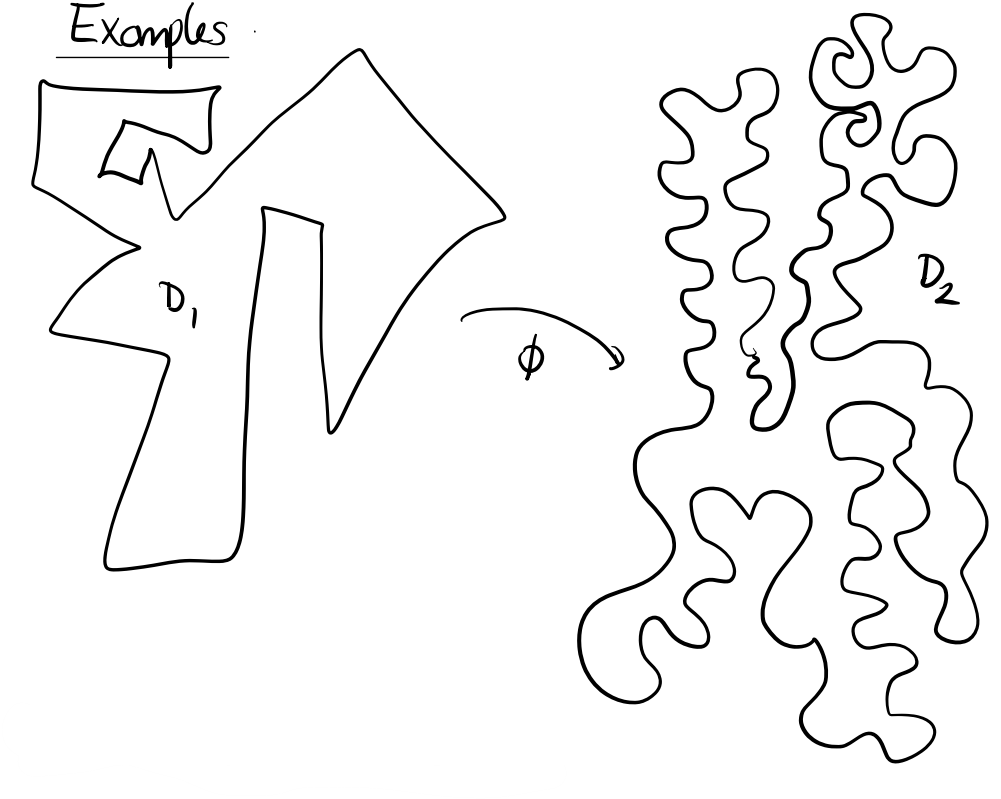
\includegraphics[width=0.5\textwidth]{LECTURE_17/graph3.png}
    \caption{Riemann Mapping Theorem}
\end{figure}
\begin{remark}
    This only proves the \underline{existence}! In general, it is not constructive!
\end{remark}

\section{Constructing Conformal Maps}

\begin{example}

    Mapping the unit disk to the upper half plane.\\
    \begin{align*}
        f = i\left(\frac{1 + z}{1 - z}\right)
    \end{align*}
\end{example}

\begin{figure}[H]
    \centering
    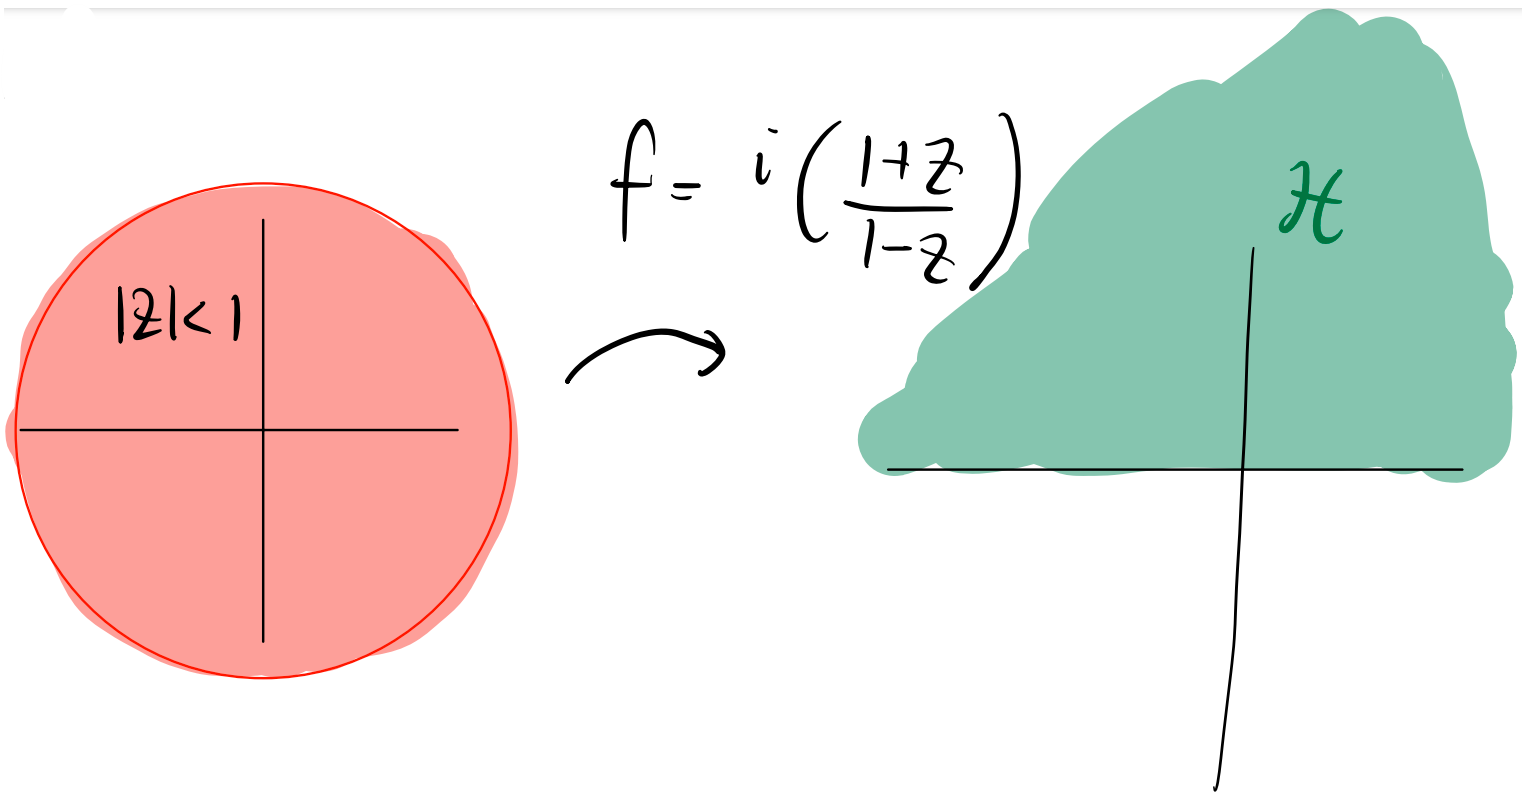
\includegraphics[width=0.5\textwidth]{LECTURE_17/graph4.png}
    \caption{Conformal Map}
\end{figure}

\begin{example}
    Mapping the upper half plane to the upper half plane plus a fraction of the lower half plane.\\
    \begin{align*}
         & h(z) = z^p \quad 0 < p < 2    \\
         & \text{Defined on } \mathbb{H}
    \end{align*}

\end{example}

\begin{figure}[H]
    \centering
    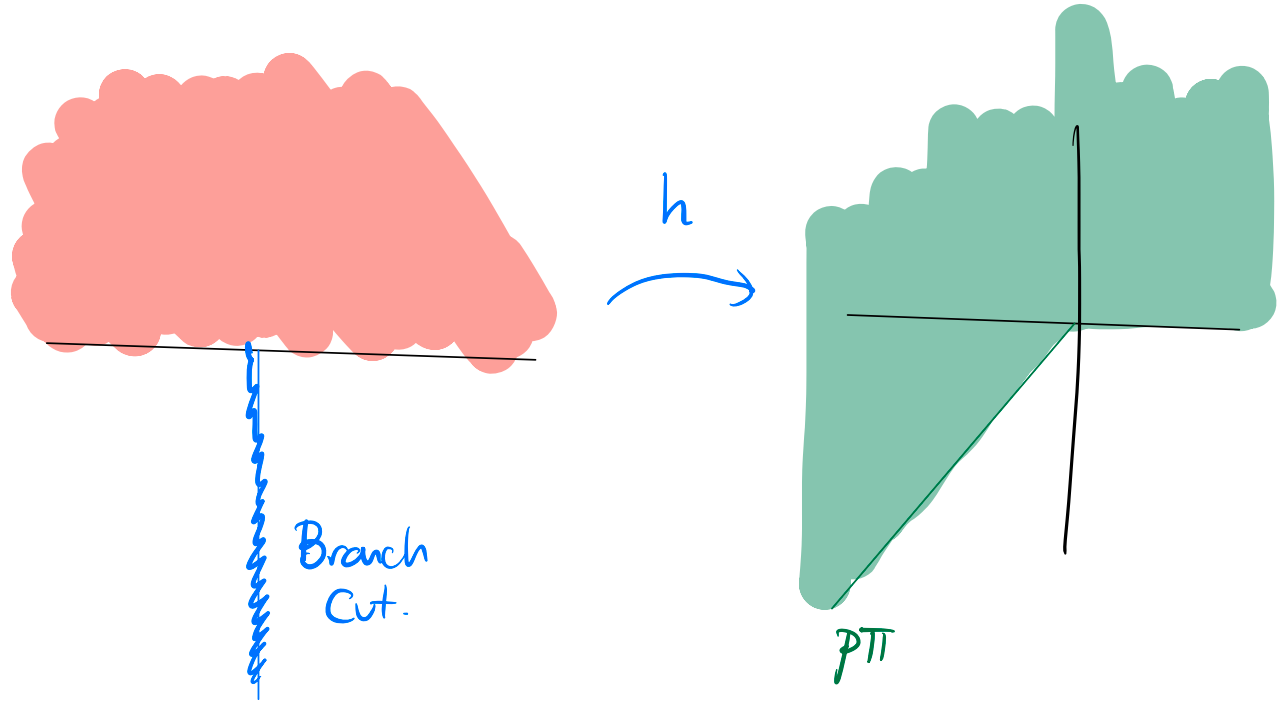
\includegraphics[width=0.5\textwidth]{LECTURE_17/graph5.png}
    \caption{Conformal Map}
\end{figure}

\section{Schwarz-Christoffel Symbols}

\begin{definition}
    This is a technique for constructing conformal maps from the upper half-plan to a polygon.
    \begin{align*}
        \mathbb{H} = \{z \in \mathbb{C} : \Im (z) > 0\} \to \text{Polygon}
    \end{align*}
\end{definition}

\begin{proposition}
    [Conformal Map from Real Numbers to Edges]
    Consider the function $f(z) = A(z - x_0)^\beta + B$ where $x_0, \beta$ are constants in $\mathbb{R}$, $0 < \beta < 2$ and $A, B$ are constants in $\mathbb{C}$. Argument chosen to lie in $(-\frac{\pi}{2}, \frac{3\pi}{2})$. \\

    Our objective is to show that $f$ maps real numbers to edges with a specific angle.
    \begin{figure}[H]
        \centering
        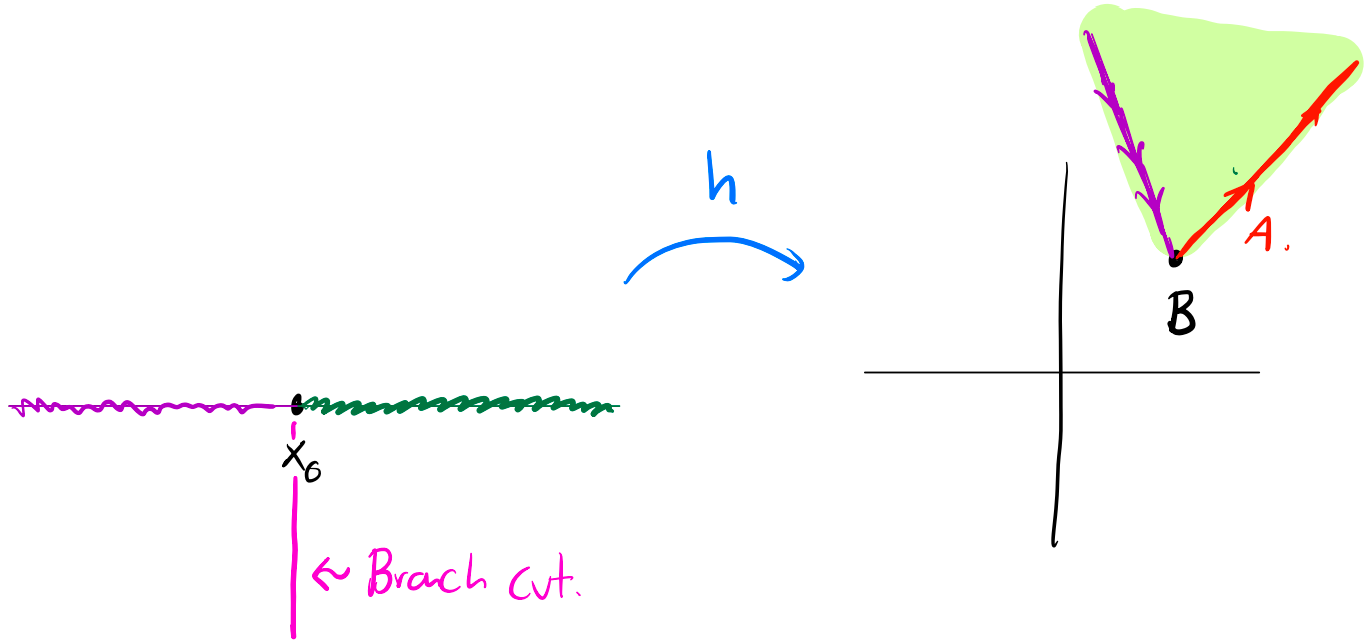
\includegraphics[width=0.5\textwidth]{LECTURE_17/graph6.png}
        \caption{Conformal Map $f$}
    \end{figure}
    We can do this by find the difference in the tangents just before and after the point $B$.\\
    Let's restrict $z$ to be real, so $z = x \in \mathbb{R}$.\\
    You can think of $f(x)$ now as a function that starts at $B$ and moves in the direction of $A$. This is true when $x > x_0$ and $\beta = 1$.\\
    \begin{figure}[H]
        \centering
        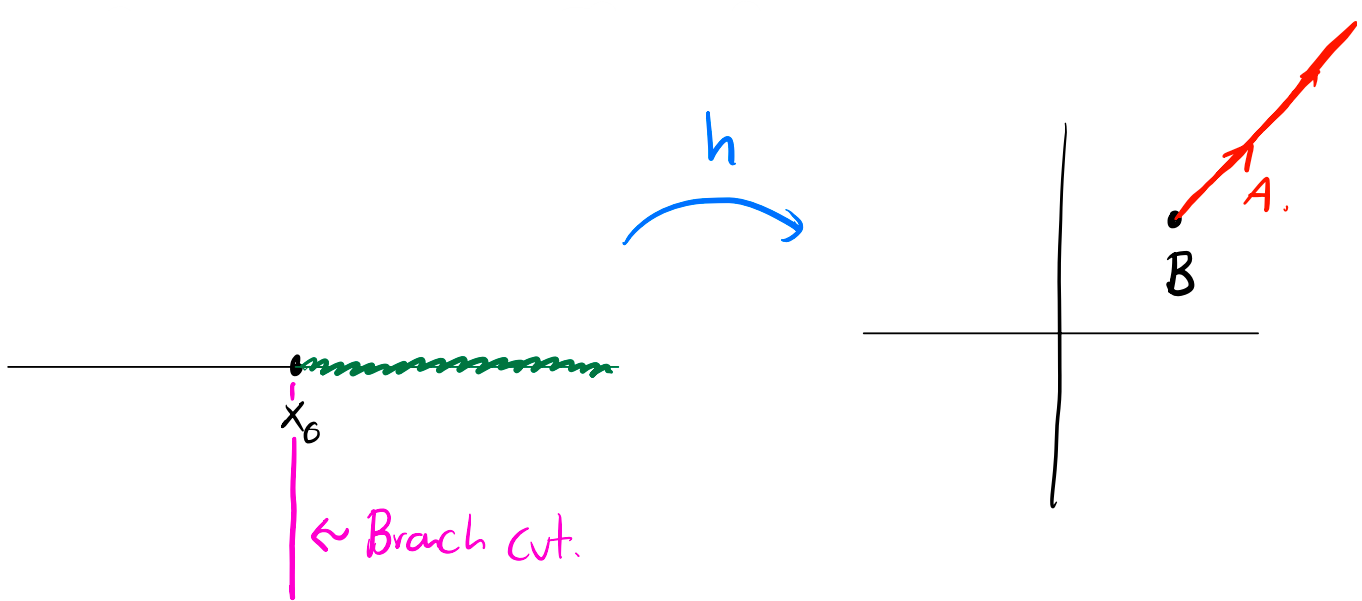
\includegraphics[width=0.5\textwidth]{LECTURE_17/graph7.png}
        \caption{Conformal Map $f$}
    \end{figure}
    Now let's write $f(x)$ in a more explicit form:
    \begin{align*}
        f(x) & = A(x - x_0)^\beta + B                                      \\
             & = Ae^{\beta \log(x - x_0)} + B                              \\
             & = Ae^{\beta \log|x - x_0| + i\beta \text{Arg}(x - x_0)} + B \\
             & = A|x - x_0|^\beta e^{i\beta \text{Arg}(x - x_0)} + B
    \end{align*}
    We can see now that $\beta$ will cause some rotation when it's not an integer.\\
    We can think of $\text{Arg}(f(z_0))$ as the angle pointing from the origin to $f(z_0)$.\\
    We can think of $\text{Arg}(f'(z_0))$ as the angle pointing from $f(z_0)$ to $f(z_0^+)$, essentially the direction of the tangent vector.\\
    With this in mind, we can find $f'(x_0^+) = B$, which the direction of the tangent vector at right after $B$.
    \begin{align*}
        f'(x)                 & = A\beta(x - x_0)^{\beta - 1}                                              \\
                              & = A\beta e^{(\beta - 1)\log|x - x_0| + i(\beta - 1)\text{Arg}(x - x_0)}    \\
                              & = A\beta |x - x_0|^{\beta - 1} e^{i(\beta - 1)\text{Arg}(x - x_0)}         \\
        f'(x_0^+)             & = A\beta |x_0^+ - x_0|^{\beta - 1} e^{i(\beta - 1)\text{Arg}(x_0^+ - x_0)} \\
        \text{Arg}(f'(x_0^+)) & = \text{Arg}(A) + (\beta - 1)\text{Arg}(x_0^+ - x_0)                       \\
                              & = \text{Arg}(A)
    \end{align*}
    The $(\beta - 1)\text{Arg}(x_0^+ - x_0) = 0$ because $x_0^+ - x_0$ is real and thus has an argument of $0$.\\
    Now we can find the tangent vector at $x_0^-$.\\
    \begin{align*}
        f'(x_0^-)             & = A\beta |x_0^- - x_0|^{\beta - 1} e^{i(\beta - 1)\text{Arg}(x_0^- - x_0)} \\
        \text{Arg}(f'(x_0^-)) & = \text{Arg}(A) + (\beta - 1)\text{Arg}(x_0^- - x_0)                       \\
                              & = \text{Arg}(A) + (\beta - 1)\pi
    \end{align*}
    Since $x_0^- - x_0$ is real and negative, it has an argument of $\pi$.\\
    Now we can find the difference in the angles of the tangent vectors at $x_0^-$ and $x_0^+$.
    \begin{align*}
        \text{Arg}(f'(x_0^+)) - \text{Arg}(f'(x_0^-)) & = \text{Arg}(A) - \text{Arg}(A) - (\beta - 1)\pi \\
                                                      & = (\beta - 1)\pi
    \end{align*}
    This means we can now map the real numbers to edges with a specific angle. We can also now see why $\beta < 2$ is required, it's because the difference between the tangents of the edges must be between $(-\pi, \pi)$.
\end{proposition}

\begin{proposition}
    [A Generalization of the Previous Proposition]
    Consider the analytic function on $\mathbb{H}$ satisfying:
    \begin{align*}
        f'(z)      & = A(z - x_1)^{\alpha_1}(z - x_2)^{\alpha_2}\ldots(z - x_n)^{\alpha_n}                                               \\
                   & \text{where } x_1 < x_2 < \ldots < x_n \in \mathbb{R} \text{ and } \alpha_1, \alpha_2, \ldots, \alpha_n \in (-1, 1) \\
        \text{Arg} & \in (-\frac{\pi}{2}, \frac{3\pi}{2})
    \end{align*}
    You can think of $\alpha_i$ as $\beta - 1$ in the previous proposition.\\
\end{proposition}

\begin{example}
    Suppose $x \in \mathbb{R}$ and $x_{j-1} < x_{j} < x_{j+1} < \ldots < x_n$. Then:
    \begin{align*}
        text{Arg}f'(x_{j}) = \text{Arg}A + \pi \alpha_{j + 1} + \ldots + \pi \alpha_n    \\
        \text{Arg}f'(x_{j+1}) = \text{Arg}A + \pi \alpha_{j + 2} + \ldots + \pi \alpha_n \\
        \therefore \text{Arg}f'(x_{j+1}) - \text{Arg}f'(x_{j}) = \pi(\alpha_{j+1})
    \end{align*}
    \begin{figure}[H]
        \centering
        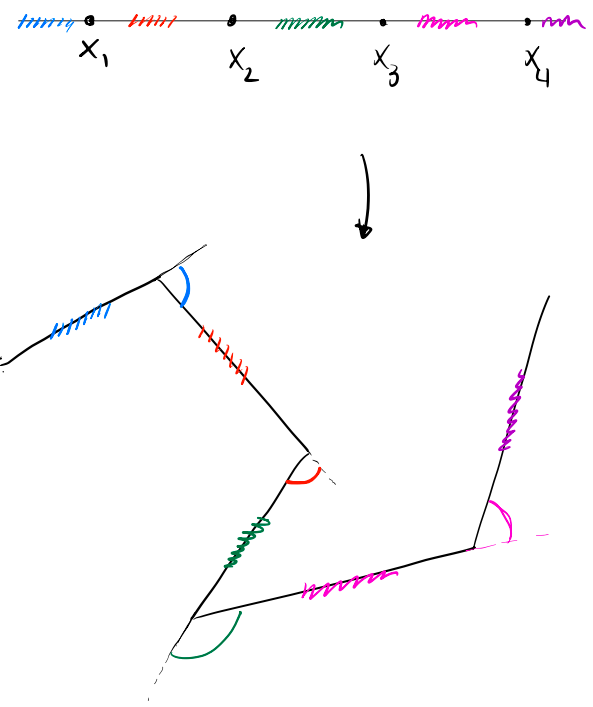
\includegraphics[width=0.5\textwidth]{LECTURE_17/graph8.png}
        \caption{Conformal Map $f$}
    \end{figure}
\end{example}

\begin{proposition}
    [Generalizing to Polygons]
    Let $P$ be a polygon with $N +1$ sides, and vertices $w_0, w_1, \ldots, w_N$. Arranged in a counter-clockwise fashion.\\
    \begin{figure}[H]
        \centering
        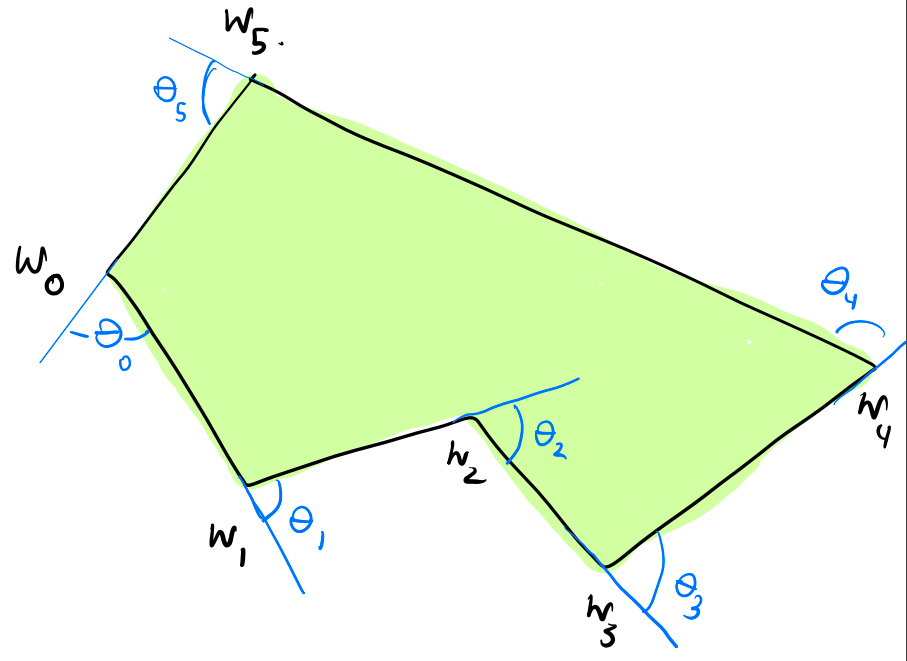
\includegraphics[width=0.5\textwidth]{LECTURE_17/graph9.png}
        \caption{Polygon $P$}
    \end{figure}

    Let $\theta_0, \theta_1, \ldots, \theta_N$ be the exterior angles of the polygon.\\
    Then we can say $\theta_0, \theta_1, \ldots, \theta_N \in (-\pi, \pi)$ and because $P$ is closed: $\theta_0 + \theta_1 + \ldots + \theta_N = 2\pi$.\\
    We know that $\alpha_j \in (-1, 1)$ so let's define $\alpha_j = -\frac{\theta_j}{\pi}$. Then:
    \begin{align*}
        \sum_{j = 0}^{N} \alpha_j = -2
    \end{align*}
\end{proposition}

\begin{theorem}
    There exists $A \in \mathbb{C}$ and real numbers $x_1 < x_2 < \ldots < x_N$ such that the Analytic function $f(z)$ on $\mathbb{H} = \{z \in \mathbb{C} : \Im (z) > 0\}$ is defined by:
    \begin{align*}
        f'(z) = A(z - x_1)^{\alpha_1}(z - x_2)^{\alpha_2}\ldots(z - x_N)^{\alpha_N}
    \end{align*}
    Which gives a 1 to 1 analytic map from $\mathbb{H}$ to the polygon $P$.
    \begin{itemize}
        \item For $j = 1, 2, \ldots, N \quad f(z_j) = w_j$. Essentially, the points $z_j | \Im (z_j) > 0$ are mapped to the inside of the polygon.
        \item $f(x) \quad x \in \mathbb{R}$ maps to the edges of the polygon.
        \item $\lim_{x \to \pm \infty} f(x) = w_0 \quad x \in \mathbb{R}$. Essentially, the points positive and negative real infinity are mapped to the left and right of the first vertex $w_0$ of the polygon.
    \end{itemize}
\end{theorem}

\begin{example}
    Find the Shwarz-Christoffel transformation taking $\mathbb{H}$ to the triangle with vertices $-a, a, i\sqrt{3}a$.
    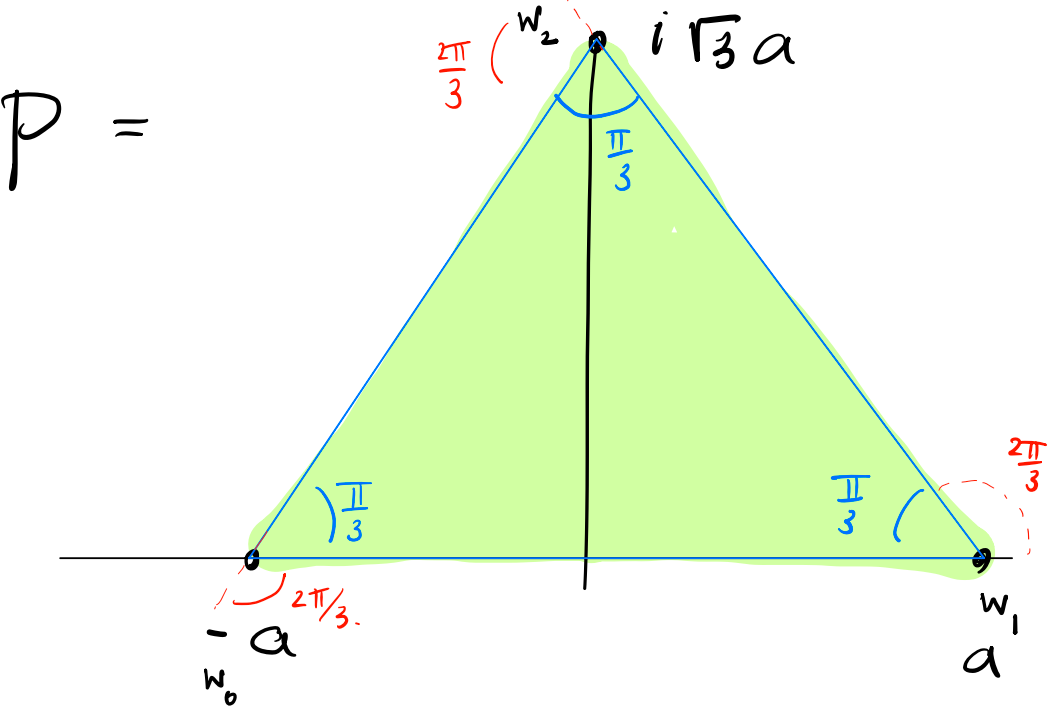
\includegraphics[width=0.5\textwidth]{LECTURE_17/graph10.png}
    The triangle has 3 sides, so $N = 2$. We choose the points $z_1 = 0, z_2 = 1$ and $z = \pm \infty$ to be mapped to the vertices of the triangle.\\
    \begin{figure}[H]
        \centering
        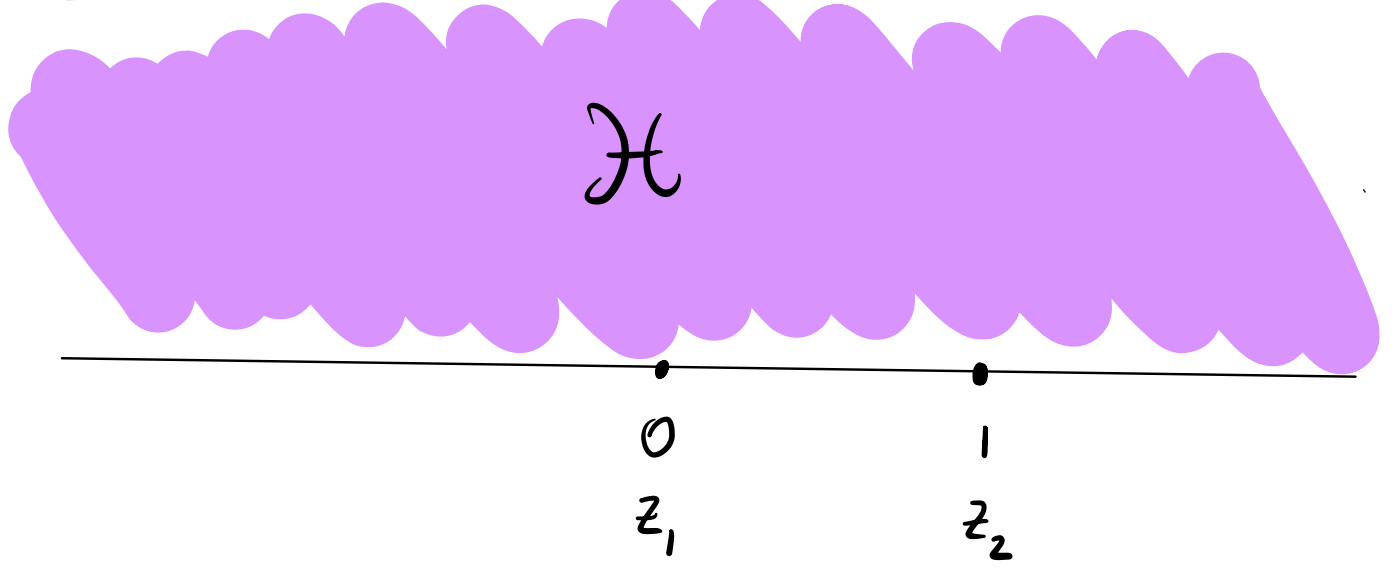
\includegraphics[width=0.5\textwidth]{LECTURE_17/graph11.png}
        \caption{Upper Half Plane with points $z_1, z_2$}
    \end{figure}
    We know that:
    \begin{align*}
        f'(z) & = A(z - x_1)^{\alpha_1}(z - x_2)^{\alpha_2} \\
        f'(z) & = A(z - 0)^{\alpha_1}(z - 1)^{\alpha_2}
    \end{align*}
    Now we can find $\alpha_1, \alpha_2$.
    \begin{align*}
        \alpha_1 = -\frac{\theta_1}{\pi} = -\frac{2\pi}{3\pi} = -\frac{2}{3} \\
        \alpha_2 = -\frac{\theta_2}{\pi} = -\frac{2\pi}{3\pi} = -\frac{2}{3}
    \end{align*}
    Now we can find $A$. Remember that any segment of the real line, as long as you don't cross the pre-image of a vertex, will have the same derivative argument as its corresponding image. So if we take the line segment $z = x \in \mathbb{R} | x < 0$ we know:
    \begin{align*}
        \text{Arg} (z)' = 0 & = \text{Arg} (f'(z))                                                        \\
                            & = \text{Arg}(A(z - x_1)^{\alpha_1}(z - x_2)^{\alpha_2})                     \\
                            & = \text{Arg}(A) + \alpha_1\text{Arg}(z - x_1) + \alpha_2\text{Arg}(z - x_2)
    \end{align*}
    Because $(z - x_1)$ and $(z - x_2)$ are real and negative, their arguments are $\pi$. So:
    \begin{align*}
        0             & = \text{Arg}(A) + \frac{2}{3}\pi + \frac{2}{3}\pi \\
        \text{Arg}(A) & = \frac{4}{3}\pi
    \end{align*}

    We can integrate to find $f(z)$.
    \begin{align*}
        f(z)      & = A\int_{1}^{z} t^{-\frac{2}{3}}(t - 1)^{-\frac{2}{3}}dt + B                       \\
        f(1)      & = A\int_{1}^{1} t^{-\frac{2}{3}}(t - 1)^{-\frac{2}{3}}dt + B                       \\
                  & = B = i\sqrt3 a                                                                    \\
        f(\infty) & = A\int_{1}^{\infty} t^{-\frac{2}{3}}(t - 1)^{-\frac{2}{3}}dt + i\sqrt3 a = -a     \\
        A         & = -a\frac{1 + i\sqrt3}{\int_{1}^{\infty} t^{-\frac{2}{3}}(t - 1)^{-\frac{2}{3}}dt}
    \end{align*}
\end{example}